% ================================================
% 文件: 02_电子管.tex
% 章节: 第3章 电子管
% 所属部分: 电子元器件与材料
% 版本: v1.0
% ================================================
% 本章目录结构（树状）:
% \chapter{电子管}
% ├── \section{热电子发射原理}
% │   ├── 直热式阴极（Directly heated）
% │   ├── 旁热式阴极（Indirectly heated）
% │   ├── 阴极构造类型
% │   └── 阴极材料（涂钍、氧化物）
% ├── \section{真空管的工作原理}
% │   ├── 屏流特性与饱和现象
% │   └── 屏极发热与散热
% ├── \section{真空管在无线电通信中的应用}
% ├── \section{二极管}
% │   ├── 特性曲线（空间电荷限制区、饱和区）
% │   ├── 整流原理
% │   ├── 滤波电路
% │   └── 负载与效率
% ├── \section{三极管}
% │   ├── 控制栅极原理
% │   └── 特性曲线
% └── \section{其他电子管类型}
%     ├── 四极管（Tetrode）
%     ├── 五极管（Pentode）
%     └── 束射四极管（Beam Tetrode）
% ================================================

\section{电子管}
\label{sec:vacuum_tubes}

电子管是早期的电子放大器件，在真空环境中工作。在无线电通信发展初期，真空管是核心器件，具有重要的历史地位和科学价值。

\subsection{热电子发射原理}
\label{sec:thermionic_emission}

利用热电子发射（Thermionic emission）可以将足够数量的电子引入到真空中。这是真空管工作的物理基础。

热电子发射的基本原理如下：若将一炽热的细导体或灯丝（Filament）放在真空中，在灯丝表面的电子获得足够的热能，当电子能量超过金属表面的逸出功（Work function）时，就能克服表面势垒发射到真空中。根据理查森-杜什曼方程（Richardson-Dushman equation），热电子发射电流密度与温度的关系为：$J = AT^2 e^{-W/(kT)}$，其中A为理查森常数，T为绝对温度，W为逸出功，k为玻尔兹曼常数。温度升高会指数级增加发射电子数量。灯丝有时就是阴极（Cathode）。
阴极必须被加热到相当高的温度才能发射电子。用来发热的电流不一定要流过发射电子的金属，即发热的灯丝可以和发射电子的阴极分开，这种真空管称为旁热式（Indirectly heated）。另一种方式是灯丝直接发射电子，称为直热式（Directly heated）。

\begin{figure}[htbp]
    \centering
    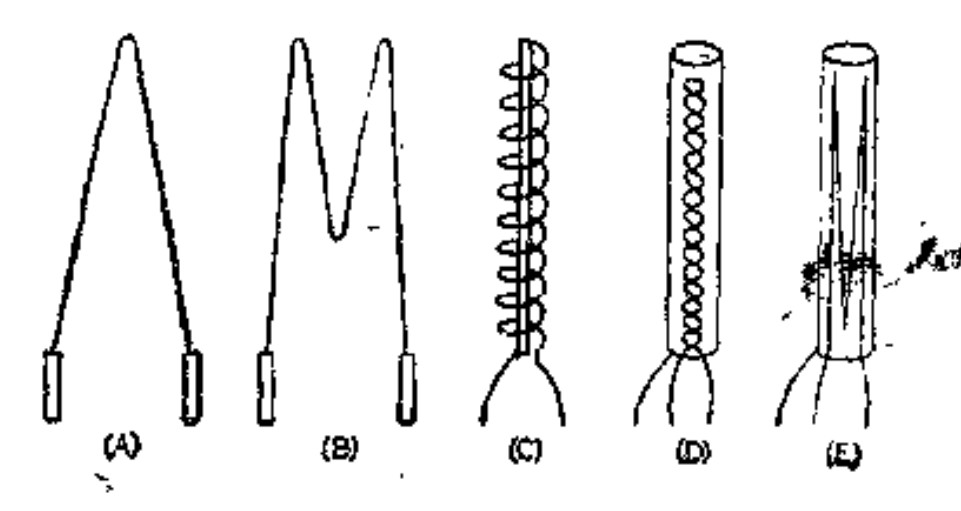
\includegraphics[width=0.8\textwidth]{Images/cathode_diagram.jpg}
    \caption{直热式与旁热式阴极结构示意图}
    \label{fig:cathode_structure}
\end{figure}

各种阴极的构造：A、B和C表示三种直热式阴极或灯丝。V形灯丝用在小接收管内，M形用在接收管和发射管内，螺旋形用在发射管内。D和E表示两种旁热式发热器构造，一种灯丝扭成圆形，另一种为M形，都用来抵消因电流流过发热体时所产生的磁场。

为实现发热电力最小而发射电子最多，阴极需采用特殊材料：
\begin{itemize}
    \item \textbf{涂钍钨阴极（Thoriated tungsten）}：在钨表面涂覆钍层，可在较低温度下发射大量电子
    \item \textbf{氧化物阴极（Oxide-coated）}：在金属基底上涂覆稀土族氧化物（如氧化钡、氧化锶），发射效率更高
\end{itemize}

氧化物阴极发射效率虽高，但只能用于较低屏压的真空管，因此主要用于接收机；涂钍钨灯丝则适用于较高电压的真空管，可用于发射管。

如真空中仅有一阴极，放射出来的大部份电子将形成云状，停留在阴极的附近。因为在空间的电子带有负电荷，在阴极的空间区域中形成一负电荷区；此负电荷区排斥靠近阴极的负电子，使其重新回到阴极上去。

设另一导体放在真空内，但不与管内的任何物相接触。若将此第二导体给予正电荷（对阴极而言），空间的电荷将被此正导体所吸引。若将电源接在此导体和阴极之间，使各得到需要的电荷，阴极放射的电子将被带正电荷的导体所吸引，形成电流再经电源而完成整个的电路。

带正电荷的导体通常都是一块金属板，或一个金属圆筒（围绕着阴极），叫它做阳极或屏极。

\subsection{真空管的工作原理}
\label{subsec:vacuum_tube_operation}

真空管与其他电气设备的显著区别在于，其电流不是通过导体传导，而是在真空中流动。只有当自由电子（Free-electrons）——即不被原子束缚的电子——被引入真空后，电流才有可能流动。

电子是带负电的微粒，在同一真空腔内，自由电子会被带正电荷的物体吸引，也会被带负电荷的物体排斥。这种吸引或排斥作用使电子在真空中运动，从而形成电流。

在真空管中因热电子发射而起的导电作用：加热电源（俗称甲电池）供灯丝发热使其到达发射电子的温度，屏极电源（俗称乙电池）使屏极对阴极保持正电位，因此屏极可以吸引阴极所发射的电子。电子到达屏极后，经外部电路返回阴极，形成完整的电流回路。

\textbf{屏流特性}：屏极所能吸引的电子数取决于屏极正电位的强度（即屏极与阴极间的电压），形成的电子流称为屏流。屏流随屏压增加而增加，但并非欧姆定律的简单比例关系。当屏压过高时，阴极发射的电子全部被屏极吸收，屏流达到饱和，不再随屏压增加而增加。

\textbf{屏极发热}：屏压与屏流的乘积等于输入真空管的电功率，这些功率主要用于加热屏极。若输入功率过大，屏极温度会升高甚至发红。热量通过辐射传递到真空管外壳，再散发到周围空气中。

\subsection{真空管在无线电通信中的应用}
\label{subsec:vacuum_tube_applications}

在无线电通信发展早期，真空管是核心技术基础：

\begin{itemize}
    \item \textbf{发射机中的作用}：产生射频功率并加以放大
    \item \textbf{接收机中的作用}：接收远处电台微弱的信号，加以放大和检波（Detect），然后放大成声音
    \item \textbf{电源转换}：将交流电转换为直流电
\end{itemize}

许多无线电通信工作离开了真空管就无法进行，因此它在无线电发展史上占有重要地位。

\subsection{二极管}
\label{subsec:diode}

二极管是最基本的真空管，包含两个电极：一极是阴极（发射电子），另一极是阳极（或称屏极，收集电子）。阴极需加热至高温才能发射电子，对于直热式阴极，灯丝本身就是阴极；对于旁热式阴极，灯丝仅用于加热独立的阴极。因为电子带负电，所以只有当屏极对阴极是正电位时才能吸引电子。若给屏极加负电位，电子将被排斥而返回阴极，真空内无电流通过。因此真空管具有单向导电性，主要用于整流和检波。

\textbf{二极管特性曲线}：以屏极电压（$V_p$）为横坐标，屏极电流（$I_p$）为纵坐标。特性曲线可分为三个区域：
\begin{itemize}
    \item \textbf{空间电荷限制区}：低屏压时，阴极附近形成负电荷云，屏流随屏压的3/2次方增加（Child-Langmuir定律：$I_p \propto V_p^{3/2}$）
    \item \textbf{过渡区}：屏流增长速率逐渐减缓
    \item \textbf{饱和区}：屏压足够高时，阴极发射的电子全部被屏极收集，屏流达到饱和，不再随屏压增加
\end{itemize}

\begin{figure}[htbp]
    \centering
    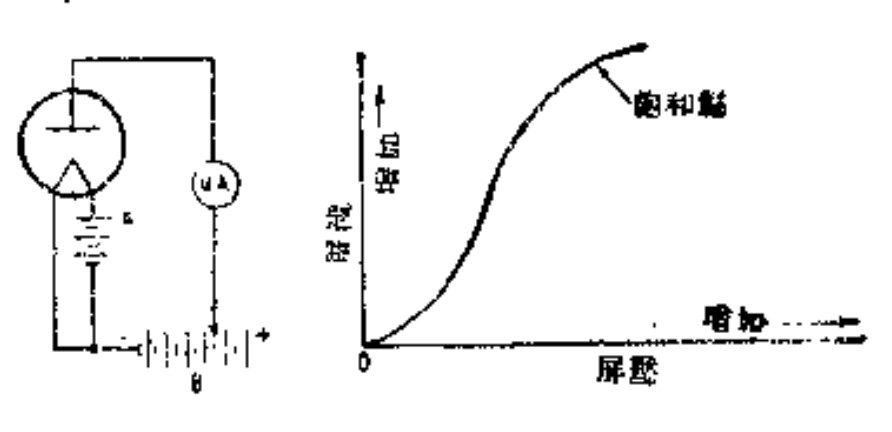
\includegraphics[width=0.8\textwidth]{Images/diode_characteristic_curve.jpg}
    \caption{真空二极管屏流-屏压特性曲线}
    \label{fig:diode_characteristic}
\end{figure}

\textbf{整流原理}：因为电流只能从真空管的一个方向流过，所以二极管可以将交流电变成直流电。当屏极对阴极为正时电流可以流过，当屏极为负时电流不能通过。只有屏极对阴极的电压为正时真空管内才有电流通过——即当变压器上端为正时的半周内才有电流流过真空管。在为负的半周中电流是不能通过真空管的。

\textbf{滤波电路}：交流电流经整流（Rectification）以后变为间歇性的直流电流（输出电流中的"驼峰"[hump]可用一滤波器使其平滑）。滤波器为感应线圈和电容器所组成，当电流流过二极管时它们将储藏起来，当二极管中变成非导体时（即没有电流流过时）将储藏的电能释放于线路中。

\textbf{负载与效率}：负荷电阻R在整流后的线路中工作；每一真空管都接有一负荷（不一定是纯电阻）。真空管的这一作用有些像发电机和变压器。在真空管线路中若不接一负荷即等于将变压器短路，将使变压器发热；所以真空管必须将它的电力输入到有用的负荷中去，而且必须使它的电力多半能输入到负荷中而不是用来作屏极发热之用。也就是说：在二极真空管的负荷上所呈现的电压应比屏极与阴极间的电压降大，也就是真空管的内电阻要比负荷电阻小。

电子管具有线性好、音质优美等优点，至今仍在音响领域有应用，但相比半导体器件，其体积大、功耗高。

\subsection{三极管}
\label{subsec:triode}

三极管是在二极管的阴极和屏极之间加入一个控制栅极（Control grid）构成的三电极真空管，是电子学发展的里程碑。

\textbf{控制栅极原理}：在真空管正常工作范围内，屏压增加时屏流也随之增加。由于空间电荷对屏极上的正电荷有抗拒效应，当屏极电压不高时不能将所有电子吸引过来。屏压愈高，克服抗拒效应的力量也愈大。若在屏极与阴极之间插入控制栅极，就可以有效地控制空间电荷：当栅极加正电压（对阴极而言）时，正电荷将中和空间负电荷，使一定屏压下到达屏极的电子增多；当栅极加负电压时，栅极上的负电荷将使空间电荷增加，使一定屏压下到达屏极的电子减少。

栅极仅控制空间电荷而不吸收电子，因此被做成网状或螺旋状，电子可以由空隙中穿过到达屏极。栅极如同一个阀门控制着屏流，实际上栅压对屏流的作用远比屏压对屏流的作用大——一定屏流的变化需要屏压变动很大才能实现，而栅压只需稍微变动即可达到同样效果。

\textbf{特性曲线}：任何真空管，栅压对屏流的效应都可用一组特性曲线（Characteristic curves）表示。当栅压为正时的曲线也可以同样画出，只需将曲线向上延长。但在多数工作情况下，常保持栅极为负，此时栅极排斥电子，没有电子到达栅极，栅极线路内没有电流；当栅极为正时，它吸收电子产生栅流，会造成电力损失。

\begin{figure}[htbp]
    \centering
    %\includegraphics[width=0.8\textwidth]{Images/triode_characteristic_curve.jpg}
    \caption{三极管特性曲线族}
    \label{fig:triode_characteristic}
\end{figure}

\subsection{其他电子管类型}
\label{subsec:other_tube_types}

\textbf{四极管（Tetrode）}：在三极管的基础上增加一个抑制栅极（Suppressor Grid），位于控制栅极和屏极之间。四极管改善了放大性能，减少了极间电容，提高了工作频率。

\textbf{五极管（Pentode）}：在四极管的基础上再增加一个抑制栅极，进一步减少二次发射效应，改善放大线性。五极管具有较高的电压放大系数和输出功率。

\textbf{束射四极管（Beam Tetrode）}：一种特殊的四极管，采用束射屏结构代替抑制栅极，通过电子束聚焦技术实现类似五极管的性能，同时具有更高的效率和更低的失真。
